\section{PDF: Structure, Complexity, Vulnerabilities}
\label{sec:pdf}

\subsection{PDF Structure}
\label{sec:pdfstructure}

\begin{figure}[t]
    \centering
    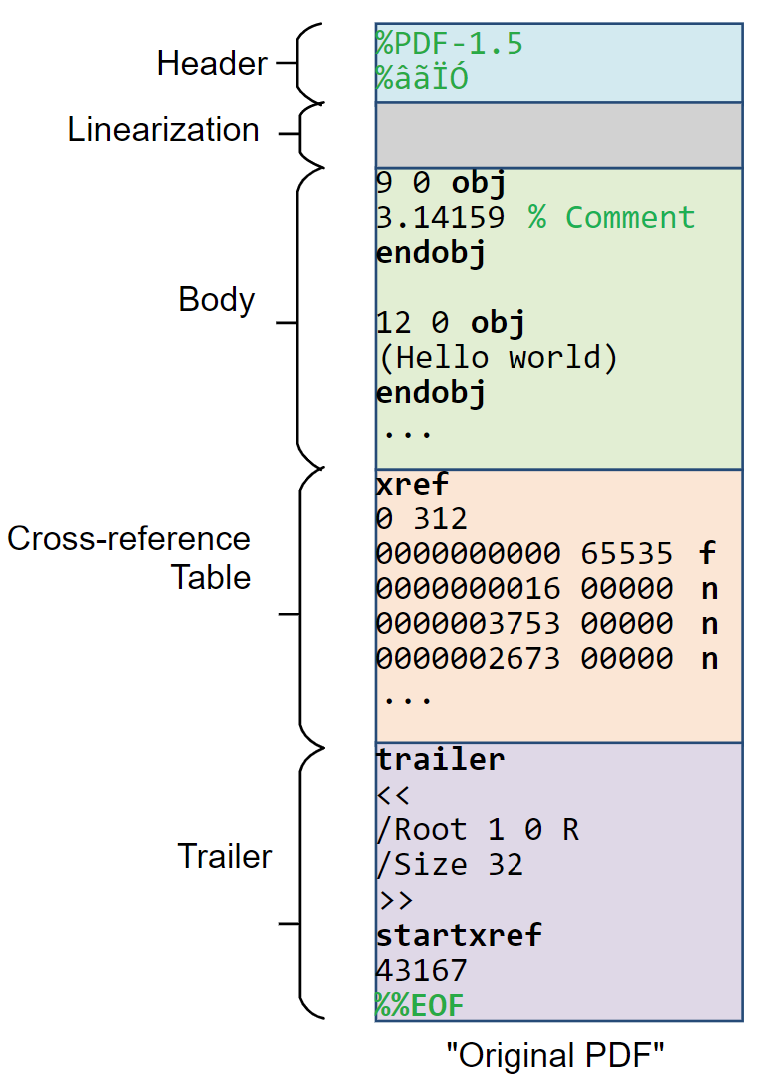
\includegraphics[width=0.65\linewidth]{figures/pdf-structure.png}
    \caption{The structure of a PDF file: labeled sections with selections of representative text.}
    \label{fig:pdf-structure}
\end{figure}

PDF is a random-access file format that contains binary 8-bit data, line-based ASCII
text data (terminated with various end-of-line sequences), and a fixed format ASCII 
data format in different sections of a single file. The overall structure of a 
traditional PDF file without any incremental updates is shown in \cref{fig:pdf-structure} and 
described below, based on the official PDF Standard.
PDF 1.5 introduced more compact file structure capabilities known as cross-reference streams 
and object streams however since this builds on the following concepts, this modern 
variation on the PDF file structure will be described later.

The PDF \emph{Header} section contains the file identification marker as an ASCII
text comment line \lstcd{\%PDF-} followed by the PDF version as ASCII digits. 
An optional second comment line (starting with \lstcd{\%})
containing at least 4 bytes above 127 in value is recommended, as it ensures 
that PDF files are not misidentified as 7-bit text files. 
All file offsets in PDF file are from the \lstcd{\%} sign in \lstcd{\%PDF-x.y}.  

The \emph{Linearization} section is an optional optimization section that enables what is commonly
known as "fast web view". This section must occur within the first 1024 bytes of a PDF and contains
data that enables a Linearized PDF aware processor to quickly display the opening page of a PDF
while the rest of a large PDF can download in the background.
Linearizatiom data is also invalidated by incremental updates (since an update might change objects
on the opening PDF page) and must therefore be checked and ignored.
%
Because not all PDF parsers support Linearization, it is a known form
of ``parser differential by design," where a \emph{parser
  differential} is a semantically meaningful difference in the result
of two document processors when run on the same document.
%
For the purposes of this paper, we will not consider Linearized PDF further.

The \emph{Body} section is where all indirect PDF objects are defined. Indirect PDF objects
are defined as those objects that have "a unique object identifier by which other objects can
refer to it (for example, as an element of an array or as the value of a dictionary entry)."
Any PDF object may be defined indirectly: integers, real numbers, strings, arrays, dictionaries, 
streams, etc. Objects are defined by their object identifier (their object number and generation 
number pair) followed by the keyword \lstcd{obj}. 
The end of every object is defined by the keyword \lstcd{endobj}.
In \cref{fig:pdf-structure}, object 9 is a real number (in ASCII) followed by a comment
(introduced by \lstcd{\%}) and this is followed by object 12 which is a PDF literal string object
(enclosed in \lstcd{(} and \lstcd{)}). The detailed syntax of PDF  
Every indirect object is reached by knowing the file offset to the start of the ASCII integer 
object number. This offset information for all indirect objects is stored in Cross-reference Tables.

The \emph{Cross-reference Table} section begins with the \lstcd{xref} keyword. For a PDF file
with no incremental updates, the next line will be a cross-reference sub-section text line comprising
two integers in ASCII (\lstcd{0 32} in this example). The first integer is an object identifier 
and in the case of an original PDF this will always be 0. The second integer is the number of
objects in the cross-reference section.

There are two sets of
objects in every PDF document: the in-use list of PDF objects and a free list
of PDF objects. Object zero is always the start of the free list as it is not
otherwise a valid object number. Each incremental update may also move objects between these two sets.
In traditional PDF each entry for an object contains a fixed length 20-byte line of text.
The first 10 ASCII digits represent the byte offset to the object, followed by a single ASCII SPACE, 
followed by 5 ASCII digits representing an object generation number. This is then followed by
another single ASCII space and the keyword \lstcd{n} for in-use objects or \lstcd{f} for free objects.
Finally the end-of-line sequence is defined to ensure that the text line entry for each object has 
a 20-byte fixed length. A parsing subtly is also that Cross-Reference sections are the only section in PDF where comments are expressly prohibited.

The \emph{Trailer} section is at the very end of every PDF file. 
It is defined as the end-of-file comment line \lstcd{\%\%EOF} immediately
preceded by the \lstcd{startxref} keyword followed by the file offset (decimal) to 
the cross-reference table in ASCII (i.e. the byte position of the \lstcd{xref} keyword 
from the the \lstcd{\%} of \lstcd{\%PDF-x.y}). Prior to this (but technically 
defined as being immediately \emph{after} the cross-reference table) is the trailer dictionary
identified by just the \lstcd{trailer} keyword, rather than the \lstcd{obj} and \lstcd{endobj}
keywords used in the PDF Body section.

\begin{figure}[t]
    \centering
    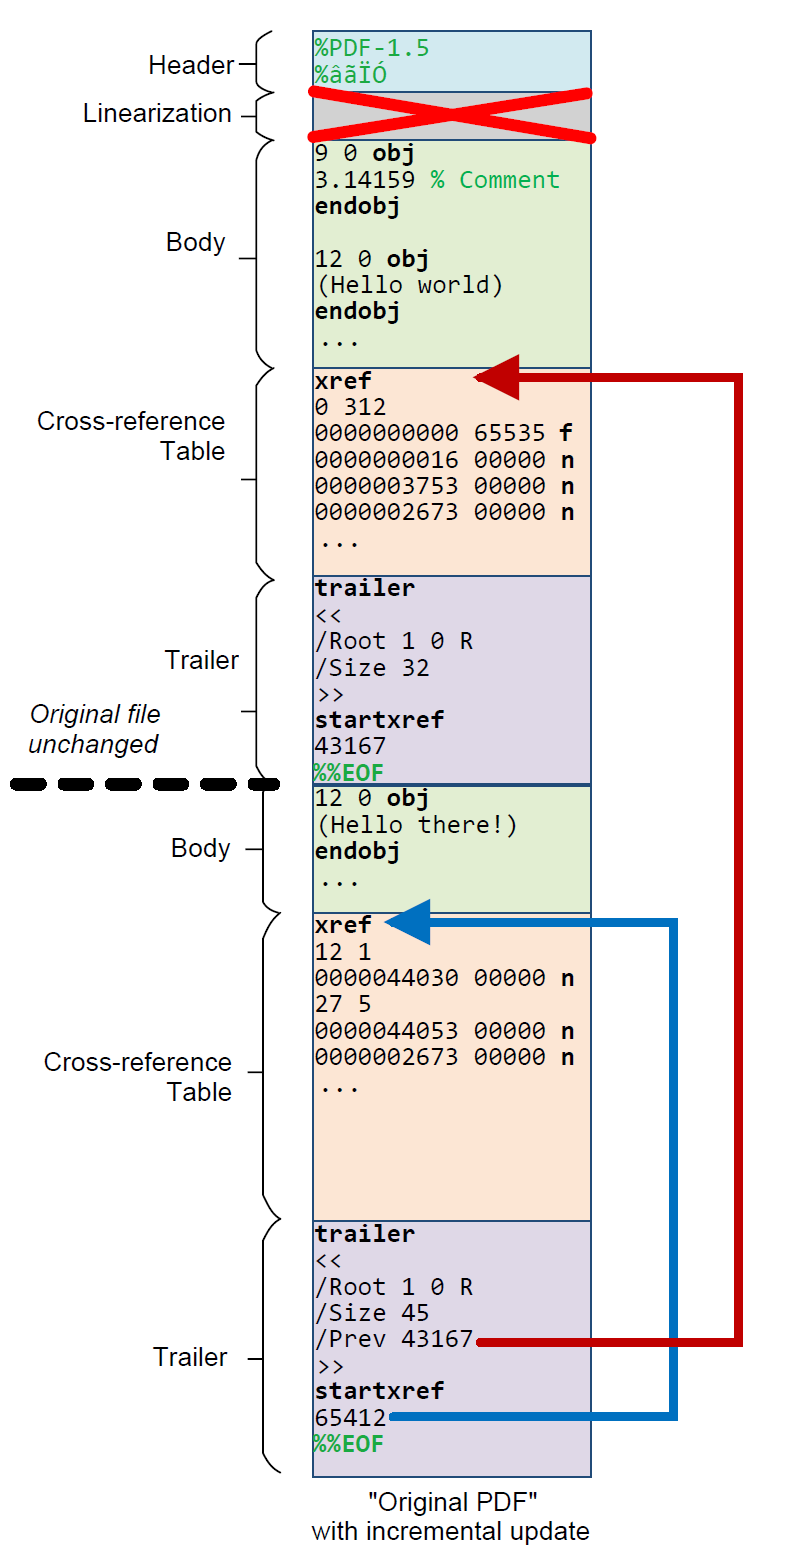
\includegraphics[width=0.65\linewidth]{figures/pdf-structure-incremental.png}
    \caption{Incrementally updated PDF File Structure.}
    \label{fig:pdf-structure-incremental}
\end{figure}

As illustrated in \cref{fig:pdf-structure-incremental}, each incremental update will 
normally append a Body, Cross-reference Table, and Trailer sections
to a PDF file with the entire original PDF remaining unchanged. The newly added incremental
update trailer dictionary will contain additional information referencing the immediately 
previous cross-reference table by byte offset. The Body section of the incremental update 
will contain any new or redefined objects. If only data in the trailer dictionary is updated then
a new Body section is not required. The cross-reference table for the incremental update
defines changes to objects made by the incremental update. This may include freeing
objects in the original PDF by adding them to the free list (the actual indirect PDF objects in
the original PDF file are not actually deleted), and/or the addition of new objects. 

\begin{figure}[t]
    \centering
    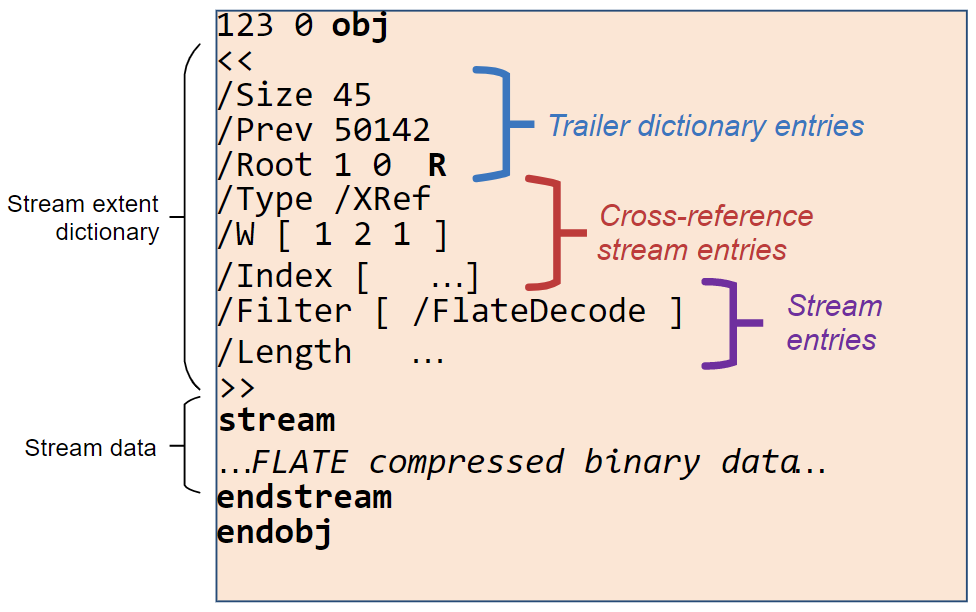
\includegraphics[width=0.65\linewidth]{figures/xrefstm.png}
    \caption{Example of a PDF 1.5 cross-reference stream.}
    \label{fig:XRefStm}
\end{figure}

As previously mentioned, PDF 1.5 introduced cross-reference streams and object streams as a means
to overcome physical file size limitations imposed by the 10-digit byte offset in the traditional
cross-reference tables.
Such files replace the cross-reference table section (including the \lstcd{xref} keyword) 
with a PDF stream object containing binary data, as shown in \cref{fig:XRefStm}. 
Like all streams in PDF, cross-reference streams may also be compressed with algorithms such as FLATE 
to further reduce file size. If a cross-reference stream is used, then the Trailer section is also no
longer used. Instead the context-defining key/value pairs are added to the stream extent dictionary of the cross-reference stream.

\begin{figure}[t]
    \centering
    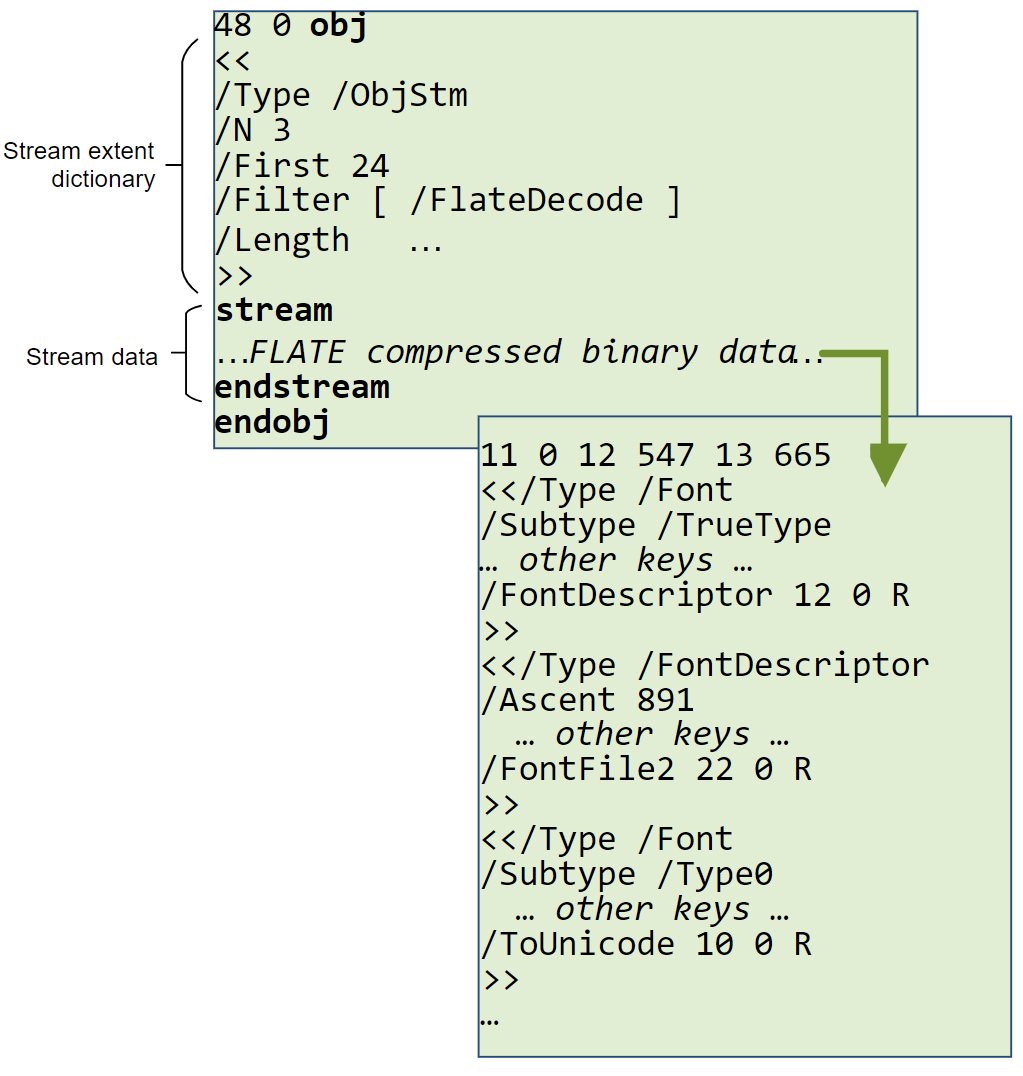
\includegraphics[width=0.65\linewidth]{figures/ObjStm.png}
    \caption{Example of a PDF 1.5 object stream and its contents.}
    \label{fig:ObjStm}
\end{figure}

Another optimization added by PDF 1.5 were object streams as illustrated in \cref{fig:ObjStm}.
It can be appreciated that a large PDF will
undoubtedly have many indirect objects and thus the repeated use of the object identifier pair with  \lstcd{obj} and \lstcd{endobj} keywords can become a significant size burden. Object streams are
compressible text streams "... in which a sequence of indirect objects may be stored, as an 
alternative to their being stored at the outermost PDF file level". 
Syntactically object streams no longer uses the \lstcd{obj} and \lstcd{endobj} keywords and replace the object identifier pair with a single object number and a byte offset within the stream. 
By using stream compression algorithms, the text-based data can be drastically reduced in size.
If object streams are used then cross-reference streams must also be used, however cross-reference 
streams may also be used by themselves with the traditional Body section.

As noted above because both cross-reference streams and object streams are standard PDF streams, they 
can benefit from stream compression. However this also means that parsers are then also  
susceptible to "ZIP bomb" attacks and handling of semantic errors (invalid stream extent dictionaries) during pre-DOM processing!

A further complication is the concept of "hybrid-reference" PDF files, where both traditional cross-reference tables and cross-reference streams co-exist in the same PDF so as to provide some semblance of support for non-PDF 1.5 aware parsers. This complication is not addressed further in this paper.

There is no limit to the number or types of incremental updates that can be added to a PDF file. Later
updates may also "undo" changes from any previous incremental updates by restoring (changing to in-use)
previously feed objects. For incremental updates, PDF object numbering 
does not have to be sequential, with skipped object numbers assumed to be on
the free list (although this is not stated explicitly in the PDF Standard).

In effect, incremental updates form a timeline of all changes made to a PDF, with parsing starting
at the end of the file with the most recent change back to the original document at the to of the file.

\subsection{Parsing PDF File Structure}
\label{sec:parsingfile}

The above paragraphs describe the physical layout of a PDF, but the processing sequence may not be so apparent. The following paragraphs describe the processing necessary to correctly parse a PDF file with incremental updates.

PDF parsing begins by locating the PDF Header as it is not uncommon for PDF files to have 
preamble bytes (such as an HTTP header, HTML or XML). The offset to the start of the PDF file 
(PDF offset zero)
within a physical file must be determined from the \lstcd{\%} sign in \lstcd{\%PDF-x.y}. 
Processing then continues by seeking to end-of-file and locating the last end-of-file marker \lstcd{\%\%EOF} in the physical file.

It is then necessary to locate the last \lstcd{startxref} keyword and the following PDF file byte offset 
to the last Cross-Reference Table in the PDF. Note also that this requires parsing \emph{backwards}
which is unnatural for many programming languages and is a proven source of parser differentials. This PDF byte offset must also be adjusted to a physical file offset by accounting for any preamble bytes prior to the PDF Header.

The parsing dialect depends on the form of the incremental update, with
traditional cross-reference tables being simpler and largely independent of
other processing. Cross-reference streams however are more complex as they are
often compressed and thus require the pre-DOM parser to "trust" the stream
extent dictionary data.

The parser must then locate either the \lstcd{xref} keyword for
traditional PDF cross-reference tables, or a cross-reference stream, identified by tokens of the form \lstcd{x y obj} . 
A parser must then determine if the PDF object is a
semantically valid cross-reference stream by further parsing the stream extent dictionary and 
validating the necessary key/value pairs and also recognizing the \lstcd{stream} keyword after the dictionary end token \lstcd{>>} and the \lstcd{endstream} keyword (see \cref{fig:XRefStm}). 

In the case of traditional PDF
cross-reference tables, after the cross reference table will be the
trailer dictionary identified by the \lstcd{trailer} keyword. 
Note that this algorithm is at
odds with the file structure as defined in the PDF Standard: the Trailer Section is defined
to contain the trailer dictionary and \lstcd{startxref} keyword, yet the parsing algorithm
requires locating the first trailer \emph{after} the end of the cross-reference table 
(versus the last trailer dictionary above the \lstcd{startxref} keyword). 
Alternatively for PDF 1.5 and later files with cross-reference
streams, the trailer dictionary keys should be in the stream extent
dictionary of the cross reference stream. 

Any previous cross-reference data is identified by the value of the \lstcd{Prev} entry in either
the trailer dictionary or the stream extent dictionary of a cross-reference stream. The
value of the \lstcd{Prev} key the byte offset to the immediately
preceding cross-reference table which, again, can either be a traditional
cross-reference table and to the start of the \lstcd{xref} keyword, or to a
cross-reference stream. This process repeats, working from the most recent incremental
update back through time to the original PDF document.

In each incremental update, the trailer dictionary is required to duplicate all keys from the previous
trailer and update accordingly. Of particular note is the \lstcd{Size} entry, which must be
one greater than the largest object number allocated in the PDF file. Objects with numbers greater
than \lstcd{Size} are defined to be the special PDF \lstcd{null} object.

Data in each cross reference table must be parsed to
identify the byte offset to the start of each PDF object, whether this be a file offset to an indirect object in a Body section, or a relative object position within an object stream (and where the object position is transformed to a byte offset within the object stream from the first line of text in the object stream). Note also that with traditional PDF cross-reference tables there is no definition for the byte offset to the end of an object, however for cross-reference streams this can be pre-determined.

\mttodo{maybe: import the type definitions}

\subsection{Root Causes of PDF Complexity}
\label{sec:rootcause}

Most data formats can be described by much simpler mechanisms;
most language processors (e.g., a Python parser) can be described and parsed by
textbook methods (e.g., the old \emph{lex} and \emph{yacc} are sufficient for
most language processors);
so what makes PDF processing so much more complex?

As described above, PDF uses random access to byte offsets to then parse lines of text,
which may then switch to binary data parsing. 
In some, but not all, cases the end of an object can be known, but in the most common case 
of traditional cross-reference tables only forward parsing can determine the end of an object. 
This gives rise to a phenomena we call \emph{cavities} where not every byte in a PDF file is parsed.
Such cavities can be used to hold data in an alternate format giving rise to polyglots, or potentially
to hold \emph{shellcode} that might be naively loaded into memory and then exploited 
in vulnerable parsers.
In addition, various descriptions in the PDF Standard require "parsing backwards" which is 
an unnatural programming language idiom. Furthermore, some explicit pre-DOM requirements
in the PDF Standard
refer to bytes \emph{before} a given byte offset and that parsers are highly unlikely to check. 
Our investigations reveal that these requirements are effectively "writer requirements" (unparsers) to
support better file reconstruction and recovery in the event of later data corruption. 
However if these requirements are never checked or enforced then it is possible to use them as attack
vectors.  
The PDF specification also requires multiple
dialects and computation (such as stream decompression).

If a PDF file accidentally or maliciously fails to adhere to this set of complex PDF file structure
rules, or a parser contains bugs, PDF parsers will typically silently attempt to recover
by reconstructing the cross-reference table information. 
This is not defined by the PDF file format Standard so 
ad-hoc algorithms are used. Typical reconstruction algorithms parse from the start of a PDF 
file, searching for indirect PDF objects (\lstcd{x y obj ... endobj}). This can clearly result
in ambiguous reconstruction of a PDF DOM and is highly likely to lead to parser differentials.

The resultant PDF DOM created by a set of indirect PDF objects forms a directed graph. 
Each PDF object is a vertex and indirect references between objects forming the directed edges. It is 
specifically \emph{not} acyclic as PDF formally defines concepts such as parent references to 
pages and other objects. This is different to many XML-based file formats because XML naturally forces hierarchical relationships via nesting of tags.

The PDF Standard defines very few explicit data integrity relationships for pre-DOM parsing. 
Our work has been to critically review the under-appreciated and under-studied pre-DOM PDF
file structure using formal methods to identify data integrity relationships that can 
ensure the PDF Trust Chain is robust prior to DOM processing.

% ------------------------------------------------------------------------------
\subsection{Vulnerabilities}
\label{sec:vulnerabilities}

% As will become even more apparent, there is a significant amount of
% parsing and computation that needs to be done \emph{pre-DOM}.

The majority of prior work researching PDF vulnerabilities start with a pre-existing PDF DOM,
completely ignoring pre-DOM parsing and processing. \todo{need citations} This work typically looks for
JavaScript streams or strings, action objects, URL strings, or file attachment objects that 
can lurk in various places throughout the PDF DOM. Machine-learning approaches so far have not  
used feature vectors based on the underlying PDF pre-DOM file structure. 
Prior work in privacy has identified that incremental updates obviously pose a risk for complete
redaction and data scrubbing workflows if not processed correctly.
Given our recent points about the \emph{PDF Trust Chain} (\cref{sec:trust-chain}), it should not 
surprise us that some PDF attack vectors involve aspects of breaking the \emph{DOM} abstraction.
i.e., the vulnerabilities occur \emph{pre-DOM}.

{\bf{Supply Chain attacks}} are generalization of {\bf{Shadow Attacks}} which were coined by Mainka 
et al. in \cite{mainkaShadowAttacksHiding2021} whereby an attacker infiltrates a workflow and 
maliciously manipulates a document in some way. This manipulation may be entirely syntactically valid. Only later in the workflow, possibly after a 
digital signature is applied or an official approval step, the malicious data is 
activated. In the case of digitally-signed documents this severely undermines confidence and trust
in digital signature technology.

{\bf{Parser Differentials}} are a real threat as attackers leverage differences in output
to present different information to different individuals, where the individual might be a human
or a machine. Parser differentials arise due to a combination of parser weaknesses, 
parser permissiveness, and unexpected input. In the case of PDF pre-DOM file structure, we have been
able to easily demonstrate parser differentials.

{\bf{Polyglots}} are a potential threat in any system or workflow which relies on different parsers
at different stages. If a firewall product determines a file to be of file type \emph{X} and then only 
scans for vulnerabilities relevant to file type \emph{X}, but later software decides the same file 
is file type \emph{Y}, an organization is then vulnerable. Polyglots arise from the creative use of
cavities, permissive implementations, 
and other blind spots in a file format specification where arbitrary data can be placed 
that does impact processing (e.g. in comments or strings, in freed or unreferenced objects, etc.).

{\bf{Denial of Service (DoS)}} is of increasing concern to the PDF industry, with many PDF services
and products utilizing cloud-based processing. In cases like large-scale automated invoice 
processing, DoS attacks can also incur addition expenses as well as inconvenience for an organization as exception-handling by human operators may be invoked.  

It should also be no surprise that due to complexity and subtleties of the PDF Standard described above,
extant data exhibits many errors in cross-reference tables and related pre-DOM context information.
To date, there has not been a comprehensive analysis of PDF file structure faults in extant data
caused by defects in PDF writers. One core reason is that there tooling is lacking that can report
all technical variations from the PDF Standard. However analysis of open-source PDF parser code bases
does highlight several permissive features related to pre-DOM processing:

\begin{itemize}
    \item deviation from the required 20-byte fixed cross-reference table entry, with support for
    19- and 21-byte variations due to additional white space or incorrect line endings;
    \item errors in byte offsets to indirect PDF objects and objects in object streams;
    \item errors with \lstcd{startxref} byte offsets;
    \item incorrect trailer dictionary data (such as \lstcd{Size}), leading to implementations 
    making their own independent decisions;  
\end{itemize}
